\chapter{Projekt i implementacja}

\section{Wykorzystane technologie}
\subsection{Python 3.8.1}
Do implementacji algorytmu został użyty Python. Jest to najpopularniejszy język programowania w domenie uczenia maszynowego. Wymagana jest wersja 3.8 lub wyższa ze względu na użycie w implementacji metod dostępnych od tej wersji.  
\subsection{PonyGE2}
PonyGE2 \cite{Fenton_2017} jest implementacją ewolucji genetycznej w języku Python. Pozwala na łatwą konfigurację parametrów ewolucji genetycznej oraz możliwość dodania własnych problemów, a także sposobów ewaluacji rozwiązań. Niestety, PonyGE2 nie jest przystosowane do bycia dołączaną jako niezależna biblioteka i nie umożliwia dostępu poprzez wygodny interfejs.

\begin{figure}[h]
	\centering{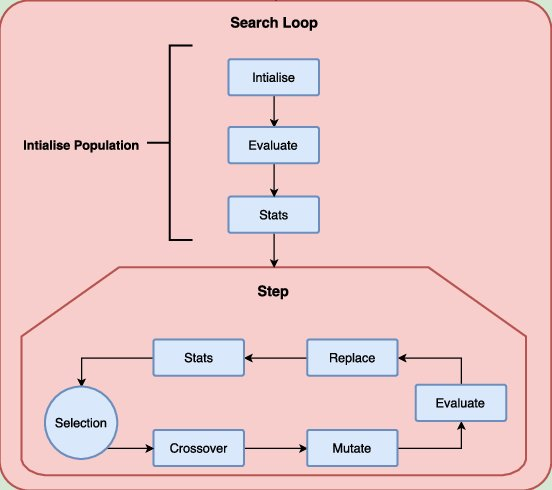
\includegraphics{PonyGE2-search-loop.jpg}}
	\caption{\label{fig:PonyGE2-search-loop}Ogólny schemat działania PonyGE2}
\end{figure}

\section{Tworzenie gramatyki procesu biznesowego}
\label{sec:businessGrammarCreation}
Projektując gramatykę procesu biznesowego, przyjęto dwa początkowe założenia. Uznano, że generowane modele muszą być łatwe do przełożenia na notację BPMN oraz nie powinny być tworzone modele niespójne strukturalnie, co pozwali na zredukowanie przestrzeni rozwiązań, jednocześnie gwarantując tworzenie niegenerujących błędów modeli.

Przy tworzeniu gramatyki procesu biznesowego ważne jest, żeby znaleźć balans, jeśli chodzi o poziom skomplikowania modelu, jaki będzie możliwy do wygenerowania, używając zaproponowanej gramatyki.  W pracy \cite{10.1007/978-3-540-69534-9_35} przeanalizowano składniki języka BPMN pod kątem częstotliwości ich stosowania. Najczęściej używanymi elementami, jeśli chodzi o bramki, są: XOR - ALBO kodowane w proponowanej gramatyce jako xor, AND - I jako and oraz pętle jako lo<0$\_$n>. Do przedstawionej dalej gramatyki dodano także bramki OR - LUB reprezentowane jako opt. Ponadto konieczne jest użycie symbolu seq, która oznacza, że aktywności następują kolejno po sobie.

Zgodnie z zaleceniami w sekcji \ref{sec:modelling} przyjmuje się, że dobrą praktyką jest, żeby model zawierał tylko jedno zdarzenie początkowe i końcowe. Z tego powodu przyjęto, że zdarzenia te są domyślnie odpowiednio na początku i końcu wygenerowanego słowa i nie są one jawnie reprezentowane w gramatyce.

W sekcji \ref{grammarCreation} opisano problemem ewolucji gramatyki dla metod opartych o krzyżowanie i mutację punktową lub n-punktową, dlatego zdecydowano się na stworzenie gramatyki pod kątem wersji tych operatorów używających fenotypu - drzewa. Lokalne przeszukiwanie często staje się słabym punktem algorytmów ewolucyjnych. Stosując wspomniane operatory, prawdopodobna jest sytuacja, że mała modyfikacja blisko korzenia może poprawić rozwiązanie, jednak jej zaistnienie wymaga wygenerowania identycznego z istniejącym poddrzewa na nowo, przez co prawdopodobieństwo wystąpienia takiej sytuacji jest niskie. Do rozwiązania tego problemu mogą służyć metody inspirowane algorytmami memetycznymi, a działające na drzewach \cite{memetic}. Dają one możliwość aplikowania lokalnych zmian bez konieczności powtórnego generowania całego poddrzewa, co pozwala na usprawnienie procesu ewolucji. Niestety, użyta biblioteka nie posiada podobnych metod lokalnej optymalizacji. Żeby w pewnym stopniu zaradzić temu problemowi, zmniejszono głębokość potrzebnego do reprezentacji modelu drzewa, jednocześnie zwiększając szanse na lokalne mutacje poprzez wprowadzenie symbolu nieterminalnego <slots>. Sprawia to, że drzewo rośnie bardziej wszerz i oprócz jednego symbolu <anygate>, którego użycie ma zapewnić tworzenie poprawnych, niepustych rozwiązań, generowane są symbole <slot>, które mogą pozostać puste lub wygenerować symbol <anygate> z 10\% prawdopodobieństwem. Przekłada się to na większą ilość lokalnych zmian na późniejszych etapach ewolucji. Lokalne przeszukiwania wspomaga także poprzez reprezentowanie bramki jako dwa odrębne symbole - <name>(<slots>). Dzięki temu w wyprowadzeniu nazwa bramki <name> jest oddzielona on jej zawartości, co sprawia, że możliwa jest zmiana nazwy bramki bez modyfikacji jej wnętrza.

Zaadresowano również konieczność odwzorowania w gramatyce częstotliwości występowania poszczególnych bramek logicznych. Zgodnie z \cite{10.1007/978-3-540-69534-9_35} połączenia i bramki XOR - ALBO, AND - I są tworzone przez większą ilość produkcji niż rzadziej występujące pętle i bramki OR - LUB. 

Zapis GE{\_}RANGE:n jest rozszerzeniem notacji zapewnianym przez PonyGE2, które umożliwia dodanie wygodne dodanie n zmiennych, czyli GE{\_}RANGE:2 w BNF oznacza 0|1|2.
Podobny jest zapis GE{\_}RANGE:dataset{\_}vars, który umożliwia dodanie ilości zmiennych odpowiadającej ich ilości w zbiorze danych w tym wypadku w liczbie aktywności w dzienniku zdarzeń. Został on dodany, dzięki rozszerzeniu standardowego, zapewnianego przez PonyGE2 parsera gramatyki.

Wszystkie bramki mają nazwy tej samej długości - 3 znaki, co ułatwia parsowanie gramatyki. Symbol startowy to <e>.

\begin{figure}[!ht]
\lstset{caption=Proponowana gramatyka procesu biznesowego, captionpos=b}
\lstset{label=src:grammar, frame=single}
\begin{lstlisting}
<e> ::= <slot><slot><anygate><slot><slot>

<anygate> ::=  <anygate><anygate> | <name>(<slots>) | {<event>}

<slot> ::= <anygate> | '' | '' | '' | '' | '' | '' | '' | '' | ''

<slots> ::= <slot><slot><anygate><slot><slot>

<name> ::= and | xor | seq | and | xor | seq | and | xor | seq | 
           and | xor | seq | and | xor | seq | lo<0_n> | lo<0_n> |opt

<event> ::= GE_RANGE:dataset_vars

<0_n> ::= GE_RANGE:5
\end{lstlisting}
\end{figure}

Model, dla którego zaprezentowanie obliczanie metryk (rys. \ref{fig:metrics_business_process}) byłby za pomocą powyższej notacji zakodowany jako:
\begin{center}
(\{a\}and(\{b\}\{c\})opt(\{b\}\{e\})\{d\}
\end{center}

Zapis lo<0$\_$n> jest nieoczywisty, jednak konieczny do reprezentacji pętli, które mogą być przerywane na innej aktywności, niż kończy się ich pojedyncza iteracja.  
Poniższy przykład pokazuje model, który ciężko opisać przy pomocy podstawowych bramek logicznych: 
\begin{figure}[H]
	\centering{\includegraphics[scale=0.4]{grammar-lop-example.png}}
	\caption{\label{fig:subcaption_example}Przykład problemu z pętlą}
\end{figure}
\noindent Jest to możliwe za pomocą słowa - lop oznacza pętle: 
\begin{center}
\{a\}and(\{b\}\{c\})\{d\}lop(\{e\}and(\{b\}\{c\})\{d\})xor(\{f\}\{g\})
\end{center}
Użycie powyższego zapisu jest poprawne, jednak kodowanie pętli w ten sposób sprawia, że powstałe słowo jest skomplikowane, a jego wyewoluowanie mało prawdopodobne. Problem ten rozwiązano, używając zapisu  lo<0$\_$n>, gdzie <0$\_$n> oznacza, ile znaków ma być pominięte w pierwszej iteracji pętli, dzięki czemu możliwe jest zakodowanie takiej pętli przy użyciu znacznie mniejszej liczb symboli, co ułatwia wyewoluowania takiego modelu. Ten sam model opisany za pomocą stworzonej gramatyki wygląda następująco:

\begin{center}
\{a\}lo1(\{e\}and(\{b\}\{c\})\{d\})xor(\{f\}\{g\})
\end{center}

\section{Projekt systemu}

\subsection{Podział na moduły}

Implementację podzielone na następujące moduły:
\begin{itemize}
  \item[•] wrappers - PonyGE2 nie jest przystosowane do zaimportowania jako biblioteka, dlatego, żeby oddzielić kod PonyGE2 od logiki odkrywania procesów biznesowych, w tym module rozszerzono lub nadpisano cześć z modułów tej biblioteki. Dodano także rozszerzenia do PonyGE2 dodające nowe, brakujące funkcjonalności.
  \item[•] fitness{\_}functions - moduł, w którym znajduje się klasa do obliczania funkcji dopasowania, która korzysta z metod w module process{\_}discovery.
  \item[•] process{\_}discovery - moduł zawiera całą logikę parsowania modelu i obliczenia metryk.
\end{itemize}


\begin{figure}[!ht]
	\centering{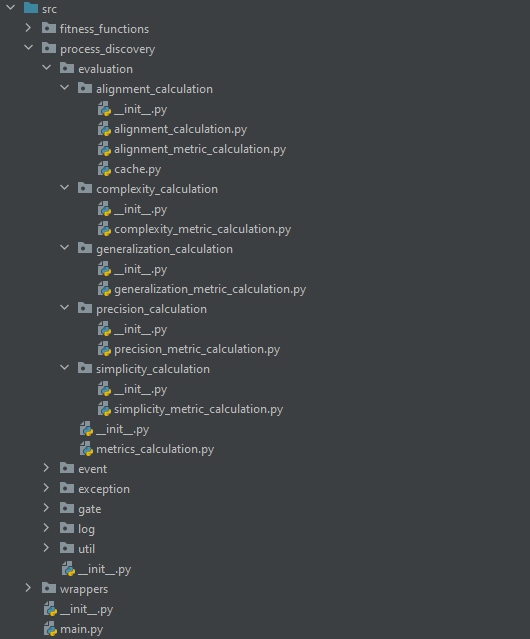
\includegraphics[scale=0.6]{Modules.png}}
	\caption{\label{fig:flow_chart}Podział na moduły}
\end{figure}

\subsection{Model}

Zdecydowano się na podział na dwie reprezentacje modelu procesu biznesowego wykorzystywane na różnym etapie procesowania. Wszystkie klasy implementują interfejs ComparableEvent pozwalający na ich porównywanie definiowanych przez nie obiektów. Aktywności są reprezentowane przez obiekty Event, które przechowują także informacje o ilości przejść w modelu przez dane zdarzenie, potrzebną do obliczenia generalizacji.  

Klasa Gate i klasy po niej dziedziczące są reprezentacją bliższą realnemu modelowi. 

\begin{figure}[h]
	\centering{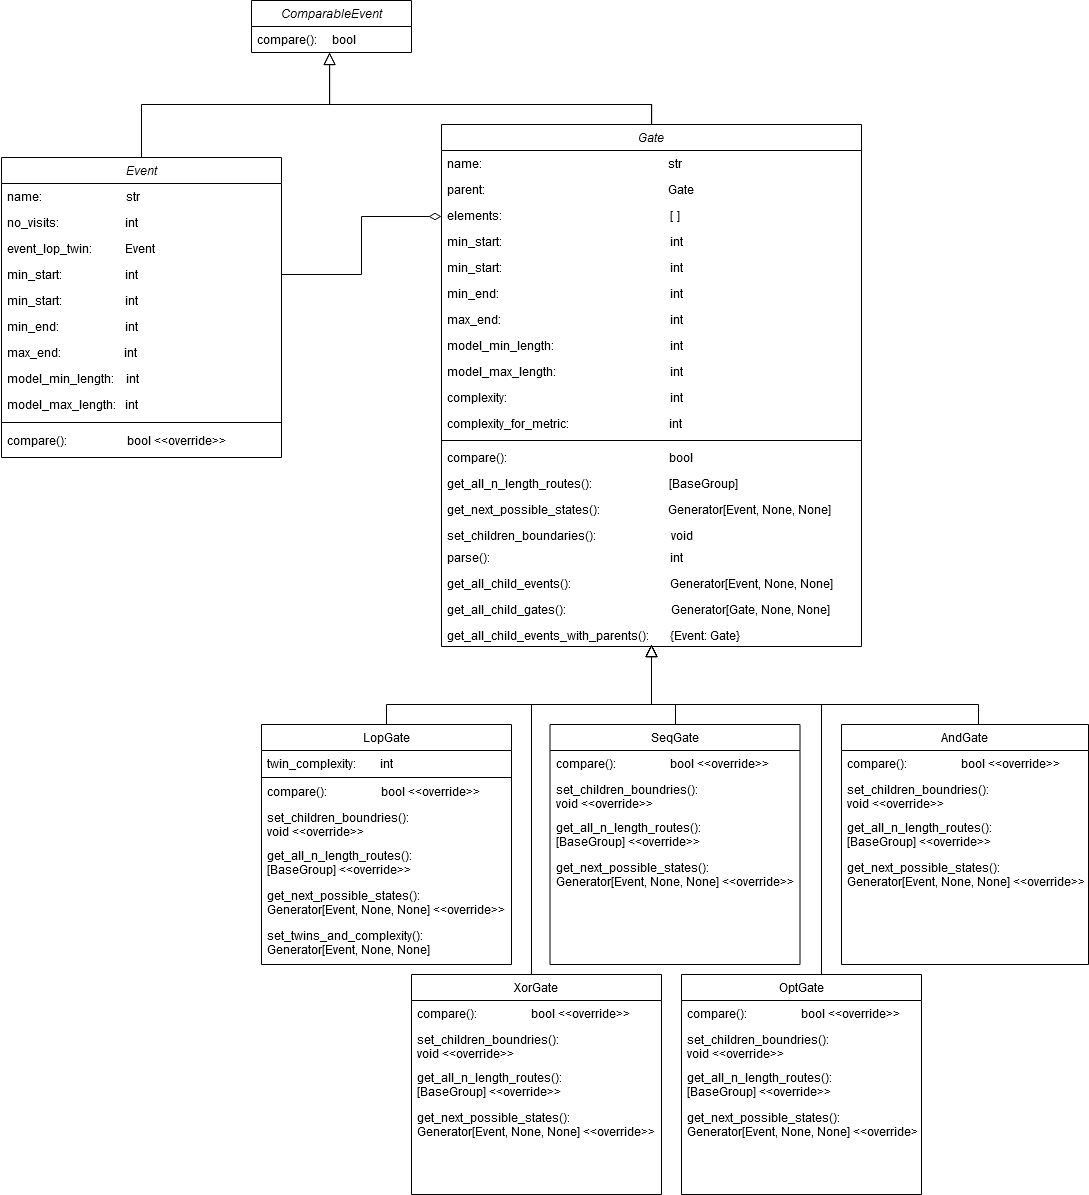
\includegraphics[scale=0.5]{GateUML.png}}
	\caption{\label{fig:subcaption_example}Gate UML}
\end{figure}

Model w formie ciągu znaków musi być zamieniony na formę, na której łatwiej będzie operować. Zakodowane zgodnie z zasadami gramatyki słowo zostaje sparsowane w metodzie parse() klasy Gate na obiekty klas po niej dziedziczących odpowiadające poszczególnym bramką logicznym. Obiekty posiadają wskaźnik na swojego rodzica, czyli bramkę - obiekt Gate, w której się znajduję oraz na bramki lub aktywności - obiekty Event, które zawierają. Przechowują też leniwie obliczaną informacja o złożoności. Najważniejsze metody, które klasy dziedziczące po Gate muszą nadpisać to:
\begin{itemize}
  \item[•] get$\_$next$\_$possible$\_$states() - zwraca jako generator możliwe kolejne aktywności, co jest potrzebne przy liczeniu precyzji.
  \item[•] get$\_$all$\_$n$\_$length$\_$routes() - zwraca możliwe ścieżki w modelu o danej długości jako tablicę obiektów BaseGroup, co jest potrzebne przy liczeniu odwzorowania
\end{itemize}

Obliczanie metryk dla klasy Gate byłoby utrudnione z uwagi na dużą ilość bramek logicznych, dlatego konieczne jest przerobienie tych obiektów na uproszczoną formę pośrednią. Są nią obiekty klas dziedziczących po BaseGroup, które dzielą się pod względem tego, czy aktywności w nich zgrupowane mogą być wykonywane w dowolnej kolejność - EventGroupParallel czy muszą być wykonywane kolejno po sobie - EventGroup. Są to wystarczające informacje do obliczenia odwzorowania, a dzięki temu algorytmu ten jest prostszy. Takie rozgraniczenie pozwala również na dodawanie nowych bramek logiczny bez konieczności zmieniana metody obliczanie odwzorowania, która jest najbardziej złożonym algorytmem występującym w programie i warto ograniczyć do minimum szansę na konieczność ewentualnych jego modyfikacji. 

\begin{figure}[h]
	\centering{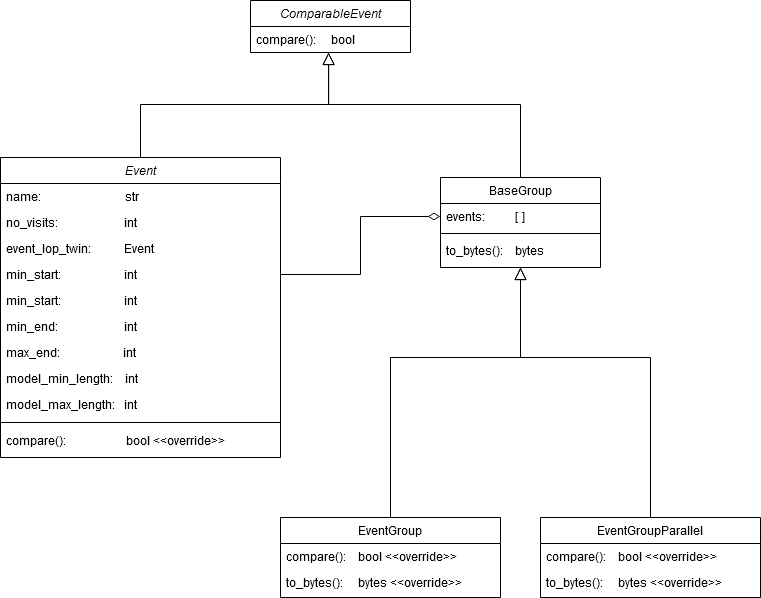
\includegraphics[scale=0.5]{EventUML.png}}
	\caption{\label{fig:subcaption_example}BaseGroup UML}
\end{figure}

Pojedyncze aktywności lub ich grupy są przechowywane jako tablica. Jedyna metoda, która musi zostać nadpisana w klasach rozszerzających BaseGroup to to$\_$bytes() potrzebna przy cachowaniu. 

\section{Implementacja}

W tej części przedstawiono listingi z pseudokodem opartym na języku Python. Tam, gdzie to konieczne pozostawiono słowa kluczowa oraz operatory tego języka.

\subsection{Ogólny schemat blokowy}


\begin{figure}[!ht]
	\centering{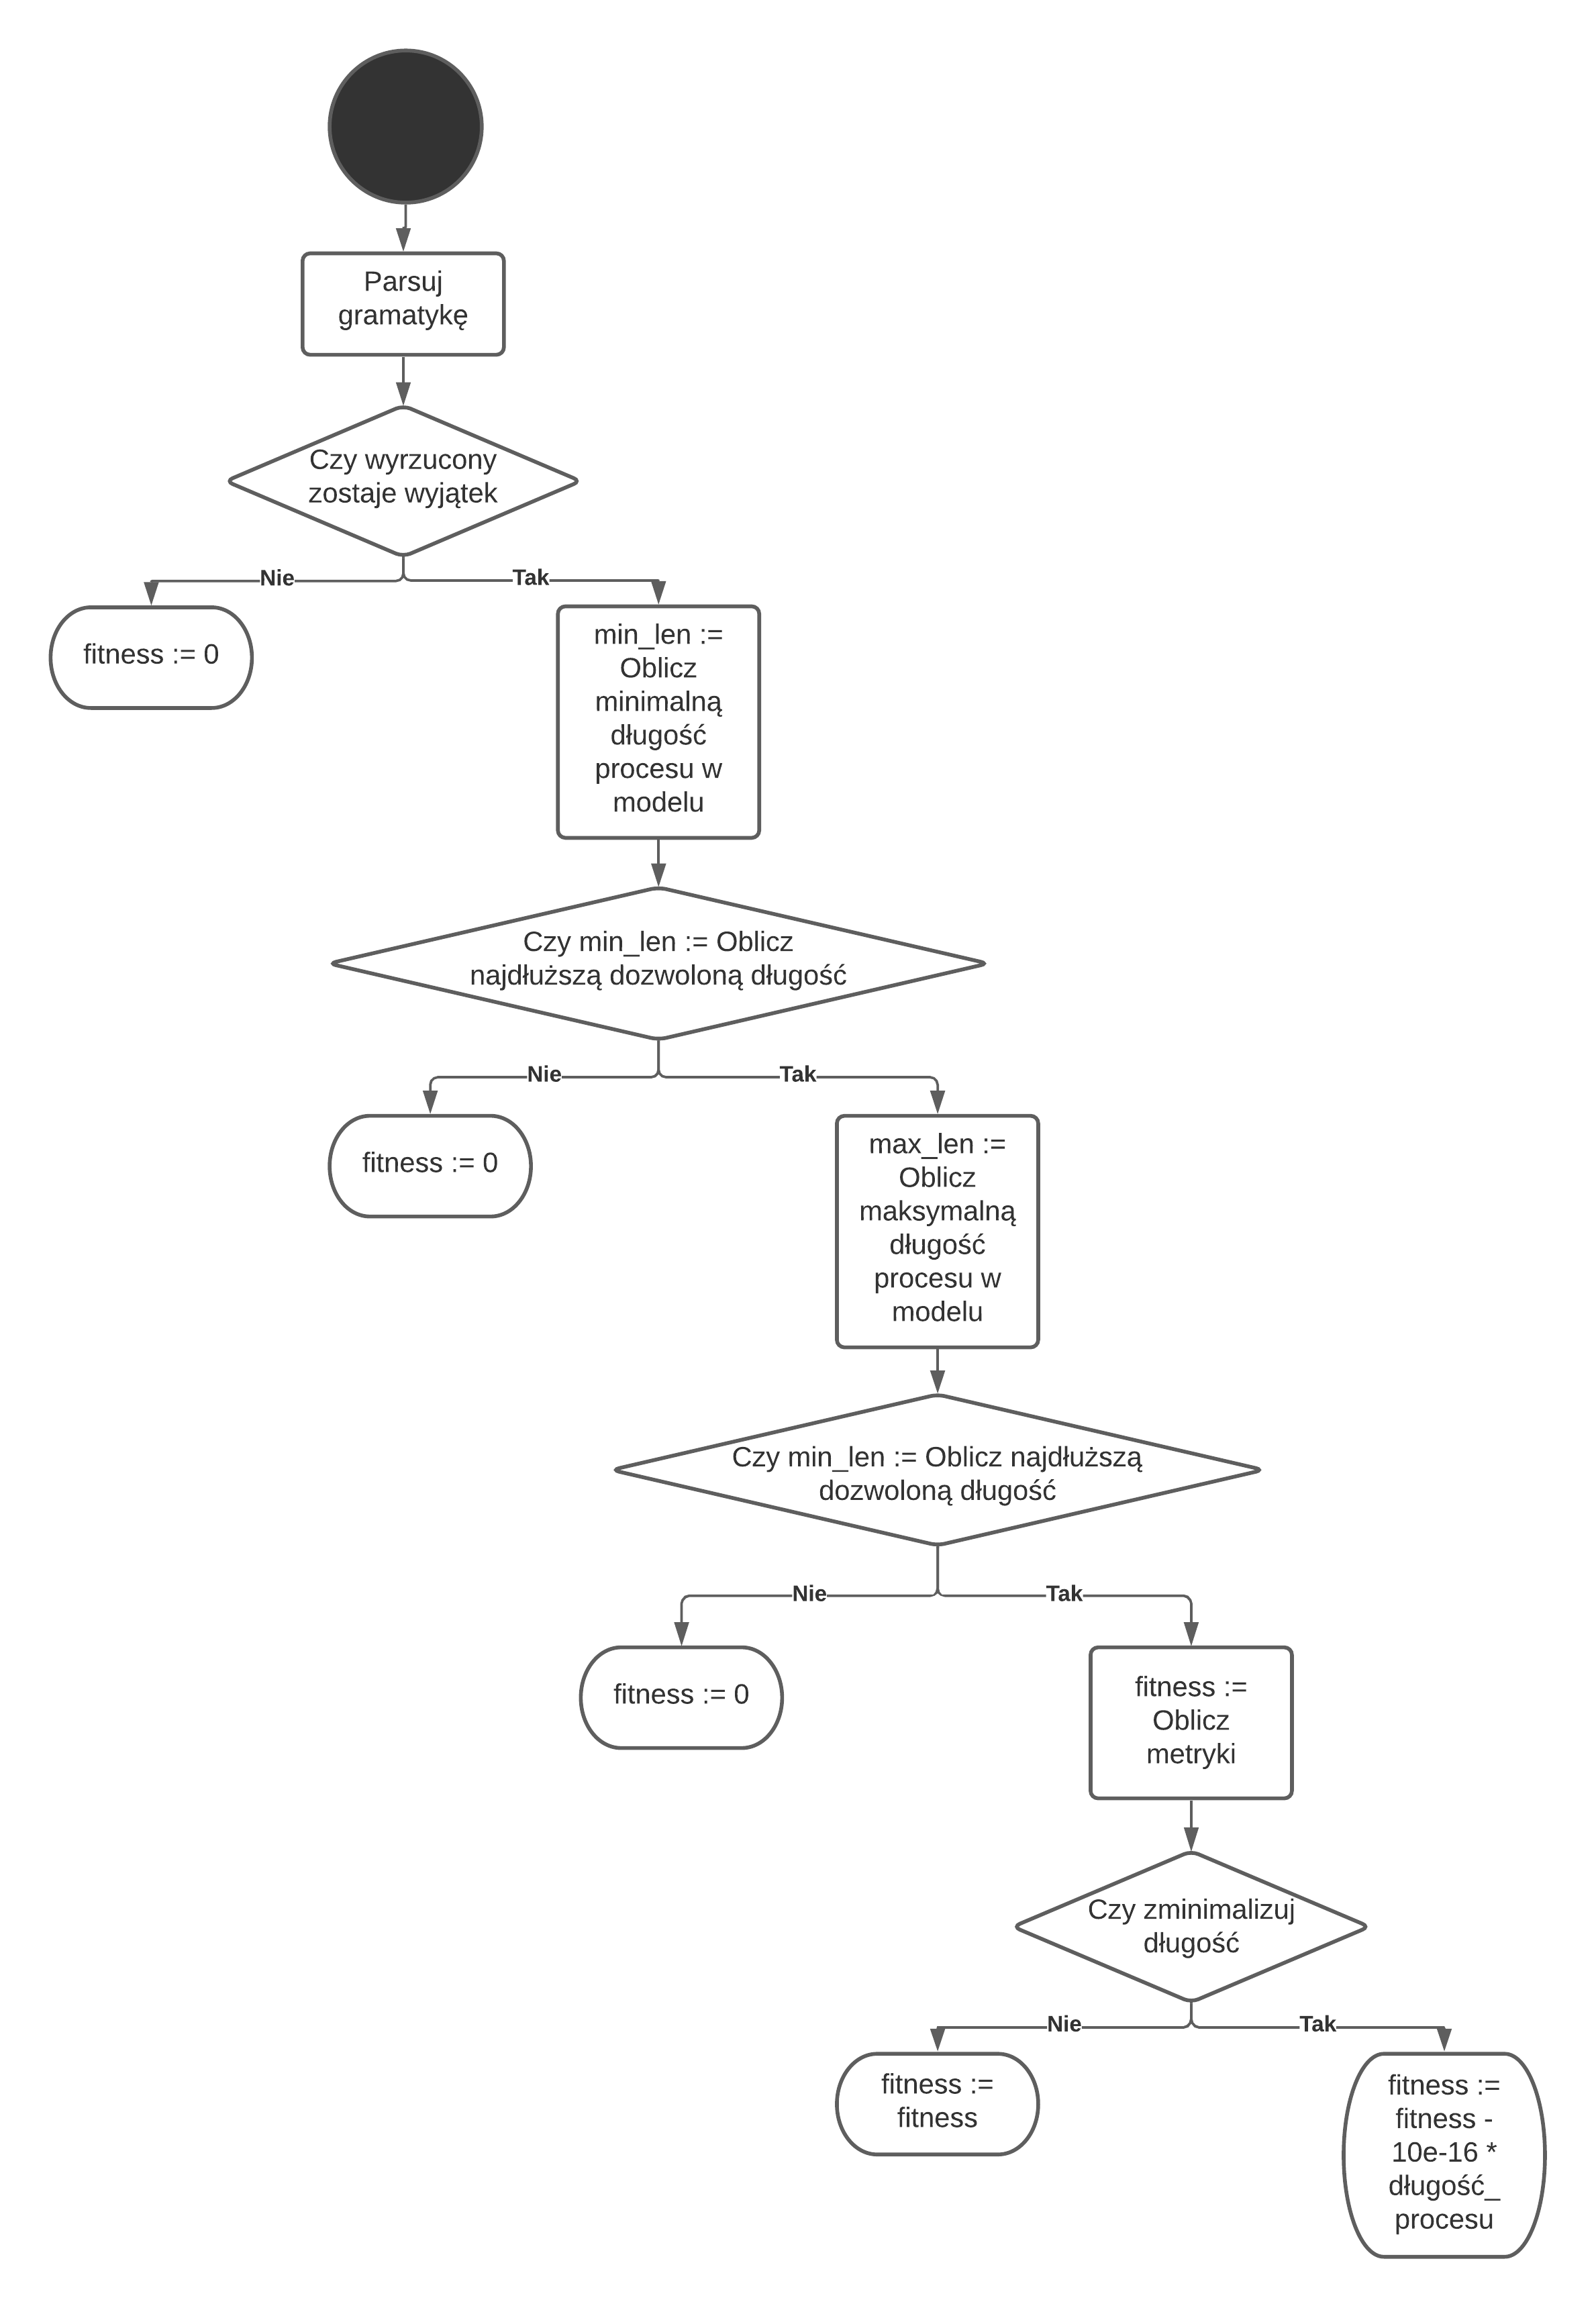
\includegraphics[scale=0.5]{OgolnySchematBlokowy.png}}
	\caption{\label{fig:flow_chart}Ogólny schemat blokowy}
\end{figure}

\subsection{Parsowanie gramatyki}
Parser pozwala na przetworzenie wyników uzyskanych na drodze ewolucji gramatycznej na postać, na której łatwiej będzie operować. Rezultaty uzyskane na drodze ewolucji gramatycznej w PonyGE2 są w formie tekstowej, z którą praca byłaby niewygodna, dlatego używamy parsera, żeby otrzymać wynik w postaci zagnieżdżonych obiektów Gate, które zawierają obiekty Event.

Metoda należy do obiektu Gate i bezpośrednio modyfikuje obiekt, na którym jest wywoływana. Argumentem metody jest wyrażenie wygenerowane w procesie ewolucji. Zwracana jest natomiast ilość przeparsowanych znaków. To na tym etapie odrzucamy też procesy, które, mimo że gramatyka pozwala na ich stworzenie, nie mają sensu z punktu widzenia biznesowego. Pozwala na ograniczenie zbędnego wykorzystania zasobów i niekontynuowanie obliczeń dla modeli, które są bezwartościowe. Na przykład takie, które pozwalają na posiadanie w jednej bramce dwóch takich samych aktywności. Parsując, korzystamy z faktu, że przy projektowaniu gramatyki wszystkie bramki logiczne zostały oznaczone 3-literowymi symbolami, a wszystkie aktywności otoczone są nawiasami klamrowymi. Pasowanie bramek można podzielić na trzy przypadki:
\begin{itemize}   
  \item[•] Bramki ,,seq'' wewnątrz bramek ,,lop'' lub ,,seq'' są redundantne i mogą zostać pominięte.
  \item[•] Pętle ze względu na konieczność specjalnego parsowanie ze względu na problem opisany w sekcji \ref{sec:businessGrammarCreation}.
  \item[•] Pozostałe przypadki.
\end{itemize}


\lstset{caption=Parser gramatyki, captionpos=b}
\lstset{label=src:passive, frame=single}
\begin{lstlisting}[escapeinside=``]
def parsuj(wyrażenie: str) -> int:

   for i in range długość_wyrażenia:
      if wyrażenie[i] == "{":
         zdarzenie := Event(wyrażenia[i + 1])
         dodaj_zdarzenie_do_aktualnie_parsowanej_bramki 
         i += 2
      elif wyrażenie[i] == ")":
         return i+1
      elif i+4 < długość_wyrażenia:
          if wyrażenie[i:i + 3] == "seq" and 
             (self.name == "seq" or self.name == "lop"):
             # pomiń zbędne bramki
             i += 3
             przeparsowane_znaki = bramka.parsuj(wyrażenie[i+4:])
             i += ilość_przeparsowanych_znaków
          else:
             if wyrażenie[i:i+2] == 'lo' and wyrażenie[i:i+3] != 'lop':  
                bramka := stwórz_nową_bramkę_Gate_typu_zgodnego_z_wyrażeniem 
                i += 3
                przeparsowane_znaki = bramka.parsuj(wyrażenie[i+4:])
                if self.name == "seq" or self.name == "lop":
                   if int(wyrażenie[i+2]) <= długość(bramka.elementy):
                      for x in bramka.elementy[int(wyrażenie[i+2]):]:
                         self.dodaj_element(x)
                dodaj_zdarzenie_do_aktualnie_parsowanej_bramki 
                i += ilość_przeparsowanych_znaków
             else:
                bramka := stwórz_nową_bramkę_Gate_typu_zgodnego_z_wyrażeniem 
                i += 3
                przeparsowane_znaki = bramka.parsuj(wyrażenie[i+4:])
                dodaj_zdarzenie_do_aktualnie_parsowanej_bramki 
                i += ilość_przeparsowanych_znaków
       else:
          wyrzuć wyjątek
\end{lstlisting}

\subsection{Obliczanie metryk}
Argumentami metody są obiekt LogInfo zawierający dane i metody dotyczące wariantów, model, czyli obiekt Gate, najkrótsza i najdłuższa dozwolona długość modelu obliczane na podstawie parametru podanego w konfiguracji programu, dzięki czemu możliwe jest zmniejszenie ilości obliczeń oraz cache. Zwracana jest natomiast średnia ważona metryk, czyli wartość funkcji dopasowania. Metryką, która nie wymaga czasochłonnego obliczenia odwzorowania, jest prostota, dlatego możemy ją obliczyć wcześniej, co przy niskim wyniku pozwala na wstępne odrzucenie części rezultatów. Łatwo można zauważyć, że jeżeli zdarzenie znajduję się w logu, a nie znajduje się w modelu, odwzorowanie nie będzie dobre. Pozwala to przerwać obliczenia, jeżeli stosunek wspólnych zdarzeń w logu i modelu jest mniejszy niż skonfigurowany parametr. Pozostałe metryki wymagają już obliczenia odwzorowania i są obliczane dla najlepiej odwzorowanej ścieżki. 

Odwzorowanie obliczane jest osobno dla każdego wariantu w logu, który jest reprezentowany jako tablica znaków. Jeśli błąd odwzorowania wynosi 0, to ilość wystąpień danego wariantu konieczna do obliczenia precyzji jest zapisywany w słowniku. Dodawana do każdej aktywności jest też ilość jej dotychczasowych wystąpień potrzebna we wzorze na generalizację.

Po uzyskaniu tych informacji dla wszystkich wariantów obliczamy średnią ważoną metryk zgodnie ze wzorami w sekcji \ref{sec:metrics-details} i uzyskujemy w ten sposób wartość funkcji dopasowania.

\lstset{caption=Obliczanie metryk, captionpos=b}
\lstset{label=src:best_result, frame=single}
\begin{lstlisting}[escapeinside=``]
def oblicz_metryki(log_info, model, najkrótsza_dozwolona_długość, 
                   najdłuższa_dozwolona_długość, cache) -> int:
                   
   lista_zdarzeń_w_modelu = model.zwróć_listę_zdarzeń_w_modelu()
   metryki['PROSTOTA'] := oblicz_metrykę_prostota(lista_zdarzeń_w_modelu, 
                                                  unikalne_zdarzenia_w_logu)
   if metryki['PROSTOTA'] < MINIMALNY_PRÓG_PROSOTY:
      return 0
   stosunek_wspólnych_zdarzeń_w_logu_i_modelu := 
      oblicz_stosunek_wspólnych_zdarzeń_w_logu_i_modelu(lista_zdarzeń_w_modelu, 
                                                        unikalne_zdarzenia_w_logu)		   
      if stosunek_wspólnych_zdarzeń_w_logu_i_modelu <
         MINIMALNY_STOSUNUK_WSPÓLNYCH_ZDARZEŃ_W_LOGU_I_MODELU:
      return stosunek_wspólnych_zdarzeń_w_logu_i_modelu/10
        
   idealnie_dopasowane_logi := pusty_słownik
   skumulowany_błąd := 0
    
   for wariant in log:
      minimalny_błąd_odwzorowania,najlepiej_dopasowane_zdarzenia,najlepsza_ścieżka := 
      oblicz_odwzorowanie_dla_jednego_wariantu(wariant, model, 
                                              najkrótsza_dozwolona_długość, 
                                              najdłuższa_dozwolona_długość, cache)
      if minimalny_błąd_odwzorowania == 0:
         idealnie_dopasowane_logi[najlepiej_dopasowane_zdarzenia] := 
         log_info[wariant].ilość_wystąpień
      dodaj_wystąpienia(lista_zdarzeń_w_modelu, najlepiej_dopasowane_zdarzenia, 
                        log_info[wariant].ilość_wystąpień)

   metryki := oblicz_metryki 
   fitness := oblicz_średnią_ważoną_metryk
   return fitness
\end{lstlisting}

\subsection{Obliczanie odwzorowania dla pojedynczego wariantu}
Procedurę obliczenia odwzorowania można podzielić następująco:
\begin{itemize}
  \item[•] Znalezienie ścieżek o długości \textbf{n} w modelu.
  \item[•] Przerobienie ścieżek na postać BaseGroup.
  \item[•] Obliczenie odwzorowania.
\end{itemize}

Argumentami metody są wariant, model, najkrótsza i najdłuższa dozwolona długość modelu oraz cache. Zwracane są natomiast minimalny błąd odwzorowania jako liczba całkowita niedodatnia, najlepiej dopasowane zdarzenia jako tablica obiektów Event oraz najlepsza ścieżka jako obiekt BaseGroup.

Algorytm obliczania odwzorowania wymaga ścieżek o stałej, określonej długość. Ważne jest, żeby jak najbardziej ograniczyć czas potrzebny na znalezienie najlepszej ścieżki, dlatego obliczanie odwzorowania rozpoczynamy o \textbf{n} równego długości wariantu. Jeśli \textbf{n} jest różne od długości ścieżki, błąd odwzorowania zawsze będzie równy przynajmniej różnicy tych wartości. Jednak wciąż może być lepszy niż aktualnie najmniejszy, więc obliczamy odwzorowanie kolejno dla ścieżek o długości n-1, n+1, n-2, n+2... aż do momentu, dopóki jest możliwe uzyskanie mniejszego błędu lub zostanie osiągnięty limit, do którego w konfiguracji zezwolono na szukanie. 

Następnie obliczane jest najwcześniejsze i najpóźniejsze wystąpienie danej aktywności w modelu, co ułatwi dalsze obliczenia. W kolejnym kroku znajdowane są wszystkie ścieżki o długości \textbf{n} w modelu i są one sortowane względem procentu wspólnych zdarzeń w modelu i logu. Możemy z tego wywnioskować jakie najlepsze odwzorowanie można otrzymać dla danej ścieżki i ewentualnie jeśli przekroczona jest dopuszczalna tolerancja błędu odwzorowania lub nie jest możliwe już zmniejszenie błędu przerwanie obliczeń dla niej.    

W końcu zgodnie z kolejnością po sortowaniu obliczane jest odwzorowanie i jeśli błąd jest mniejszy niż aktualnie najmniejszy, zamieniane są wartości minimalnego błędu odwzorowania, najlepiej dopasowane zdarzenia i najlepsza ścieżka, a jeśli błąd wynosi 0, algorytm jest przerywany i te wartości są zwracane.

\lstset{caption=Obliczanie odwzorowania dla jednego wariantu, captionpos=b}
\lstset{label=src:best_result, frame=single}
\begin{lstlisting}
def oblicz_odwzorowanie_dla_jednego_wariantu(wariant, model, 
                                            najkrótsza_dozwolona_długość, 
                                            najdłuższa_dozwolona_długość, cache):
   dłogość_wariantu := oblicz_długość(wariantu)
   n := dłogość_wariantu
   i := 1
   minimalny_błąd_odwzorowania := -(dłogość_wariantu + model.minimalna_długość)
   najlepiej_dopasowane_zdarzenia := []
   najlepsza_ścieżka := []
   dolny_limit_osiągnięty := False
   górny_limit_osiągnięty := False
   
   while not (dolny_limit_osiągnięty and górny_limit_osiągnięty):
      if n >= min(oblicz_maksymalną_dozwoloną_długość(dłogość_procesu), 
                  dłogość_procesu - minimalny_błąd_odwzorowania):
         górny_limit_osiągnięty := True
         n += (-i if i % 2 == 1 else i); i += 1
         continue
      if n <= max(oblicz_minimalną_dozwoloną_długość(dłogość_wariantu), 
                  dłogość_wariantu + minimalny_błąd_odwzorowania):
         dolny_limit_osiągnięty := True
         n += (-i if i % 2 == 1 else i); i += 1
         continue
         
      if najkrótsza_dozwolona_długość <= n <= najdłuższa_dozwolona_długość:
         ustaw_najwcześniejsze_i_najpóźniejsze_wystąpienie_zdarzenia(model, n)
         ścieżki = model.znajdź_wszystkie_ścieżki_długości_n(n, wariant)
         if ścieżki istnieją:
            for ścieżka in ścieżki:
               procent_wspólnych_zdarzeń := oblicz_procent_wspólnych_zdarzeń_
                  w_modelu_i_logu(ścieżka, wariant)
               if procent_wspólnych_zdarzeń >= 1 - TOLERANCJA_BŁĘDU_ODWZOROWANIA:
                  dodaj sćiezkę do lista_ścieżek_do_obliczenia
            posortowane_ścieżki := posortuj lista_ścieżek_do_obliczenia
            for ścieżka in posortowane_ścieżki:
               if procent_wspólnych_zdarzeń <= 1 + minimalny_błąd_odwzorowania /
                  długość_wariantu:
                  break
               błąd_odwzorowania, najlepiej_dopasowane_zdarzenia :=
               oblicz_odwzorowanie(ścieżka, wariant, cache)
               if błąd_odwzorowania > minimalny_błąd_odwzorowania:
                  minimalny_błąd_odwzorowania := błąd_odwzorowania
                  najlepiej_dopasowane_zdarzenia := dopasowane_zdarzenia
                  najlepsza_ścieżka := scieżka
               if błąd_odwzorowania == 0:
                  return minimalny_błąd_odwzorowania, najlepiej_dopasowane_
                         zdarzenia, najlepsza_ścieżka
      n += (-i if i % 2 == 1 else i); i += 1
   return minimalny_błąd_odwzorowania, najlepiej_dopasowane_zdarzenia, 
          najlepsza_ścieżka
\end{lstlisting}

\subsection{Wyszukiwanie w modelu ścieżek o określonej długości}

Łatwiejszym niż obliczenie odwzorowania dla modelu składającego się z bramek logicznych jest znalezienie najpierw w modelu wszystkich ścieżek o określonej długości i następnie jego obliczenie dla nich. Algorytm służący do tego jest kolejno wywoływane dla wszystkich bramek - podmodeli, a następnie na podstawie ścieżek znalezionych w podmodelach są tworzone ścieżki dla całego modelu. Implementacja różni się w zależności od przeszukiwanej bramki logicznej. Poniżej zaprezentowano przykład dla bramki ,,and''.  

Argumentami metody długość szukanej ścieżki oraz wariant jako tablica znaków potrzebny wyszukiwanie ścieżek dla obiektu LopGate. Zwracana jest natomiast lista wszystkich ścieżek o określonej długość jako obiekty BaseGroup, a w przypadku błędu None.

Bramki mogą zawierać różną ilość elementów, dlatego należy obliczyć minimalne i maksymalne długości, czyli ilość zdarzeń dla wszystkich dzieci. Jeśli dziecko jest obiektem Event, wtedy dodawane jest bezpośrednio do listy rezultatów. W innym wypadku, kiedy jest obiektem Gate, na podstawie długości dzieci obliczany jest dolny i górny limit długości, dla jakich zostanie dla danego elementu wywołana metoda znajdź{\_}wszystkie{\_}ścieżki{\_}długości{\_}n. Dzięki temu może znacznie ograniczyć ilość długości, dla jakich trzeba przeszukiwać podmodele. Wszystkie znalezione ścieżki są dodawane do listy, a całość do globalnej listy. 

Rezultat nie może być jednak zagnieżdżoną listą, więc musi ona zostać przerobiony na listę jednowymiarową rozwiązań. Każda lista składa się 2-wymiarowej listy ścieżek dla każdego elementów modelu. Ścieżki każdego podmodelu są łączone ze ścieżkami kolejnych podmodeli każda z każdą, żeby utworzyć możliwe przejścia dla całego modelu. Celem jest znalezienie tylko tych o długości \textbf{n}, więc pozostałe odrzucamy. Na końcu, jako że jest to bramka ,,and"" wszystkie ścieżki o długości większej niż 1 są opakowywane w EventGorupParrallel, żeby zachować informacje o tym, ze zdarzenia mogą być wykonywane w dowolnej kolejności.
\clearpage

\lstset{caption=Wyszukiwanie procesów o długości n, captionpos=b}
\lstset{label=src:get_n_length, frame=single}
\begin{lstlisting}[escapeinside=``]
def znajdź_wszystkie_ścieżki_długości_n(n, wariant) -> [BaseGroup]:
   if n == 0:
      return []
   if self.minimalna_długość_modelu < n or n < self.maksymalna_długość_modelu:
      return None

   minimalne_długości := self.oblicz_minimalne_długości_dzieci()
   maksymalne_długości := self.oblicz_maksymalne_długości_dzieci()
   globalna_lista := []

   for element in self.elementy:
      lokalna_lista := []
      if isinstance(element, Event):
         lokalna_lista.dodaj(elem)
         minimalne_długości.usuń_na_pozycji(0)
         maksymalne_długości.usuń_na_pozycji(0)
      else:
         dolny_limit, górny_limit := 
         self.oblicz_docelowy_zakres(n, globalna_lista, minimalne_długości, 
                                     maksymalne_długości)
         for i in range(dolny_limit, górny_limit + 1):
            try:
               wszystkie_ścieżki_dziecka_o_długości_n := 
               element.znajdź_wszystkie_ścieżki_długości_n(i, wariant)
            except ValueError:
               return None
            if wszystkie_ścieżki_dziecka_o_długości_n is not None:
               loklana_lista.dodaj(wszystkie_ścieżki_dziecka_o_długości_n)

         if lokalna_lista:
            globalna_lista.dodaj(lokalna_lista)

   ścieżki = []
   if globalna_lista:
      for element in spłaszcz_listę(globalna_lista):
         if self.sprawdź_długość(n, elem):
            if n == 1:
               ścieżki.dodaj(element[0])
            else:
               ścieżki.dodaj(EventGroupParallel(element))
   if ścieżki:
      return ścieżki
   else:
      return None
\end{lstlisting}

\subsection{Obliczanie odwzorowania}
Pomysł zaczerpnięty z algorytmu Needlemann-Wunsch \cite{ea252fd3937a4a309a5e07e61e5531a7}, który jest uogólnieniem odległości Levenshteina dla dowolnych wartości błędów. Tworzymy macierz o wymiarach długość modelu i długość logu, w której obliczana jest najmniejsza suma błędów. Rozwinięty o możliwość przeszukiwania modelu rekurencyjnie oraz o możliwość podawania listy równoległych zdarzeń.

Podstawowy algorytm można opisać za pomocą czterech kroków dla każdego zdarzenia:  
\begin{enumerate}
  \item Oblicz wartość w poprzednim wierszu i kolumnie dodać błąd ,,odwzorowanie'' lub ,,brak odwzorowania''.
  \item Oblicz wartość w poprzednim wierszu dodać błąd ,,przerwa''.
  \item Oblicz wartość w poprzedniej kolumnie dodać błąd ,,przerwa''.
  \item Wybierz najmniejszą wartość.
\end{enumerate}

\begin{figure}[h]
	\centering{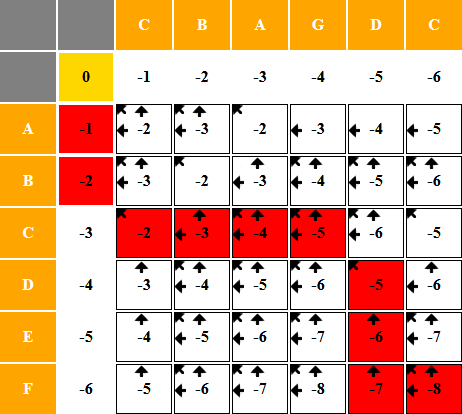
\includegraphics[scale=0.8]{needlemann-wunsch-algo.png}}
	\caption{\label{fig:algo_example}Klasyczny algorytm Needlemann-Wunsch}
\end{figure}


Argumentami metody model jako obiekt Gate oraz wariant jako tablica znaków. Zwracane są natomiast ostatni wiersz, który zawiera błąd odwzorowania modelu oraz pośrednie błędy dla wszystkich zawsze zaczynając od pierwszego zdarzenia możliwych długości wariantu, co jest potrzebne, jeśli model zawiera podmodele oraz najlepiej dopasowana ścieżka. Metoda opakowana jest w metodę, która jeśli dla danego modelu i wariantu zostało już obliczone odwzorowanie, zwraca rozwiązanie z cache bez powtarzania obliczeń.

Zgodnie z \ref{sec:alignment-calculation} brakujące zdarzenie to błąd wynosi 1, a jeśli się nie zgadzają - 2. Stworzona macierz jest inicjalizowana zerami, a następnie pierwsza kolumna jest wypełniana stosownymi wartościami błędu. Są trzy opcja normalne obliczenie zgodne z klasycznym algorytmem, a także sytuacja, w której model zawiera podmodele, gdzie algorytm jest powtórnie wywoływany dla podmodelu i dla wszystkich zawsze zaczynając od pierwszego zdarzenia możliwych długości wariantu lub gdy zawiera zdarzenia równoległe - EventGroupParallel wtedy stosujemy inny algorytm, który bezpośrednio porównuje wszystkie zdarzenia w wariancie ze zdarzeniami w obiekcie EventGroupParallel. 
     
\lstset{caption=Obliczanie odwzorowania, captionpos=b}
\lstset{label=src:alignment_calculation, frame=single}
\begin{lstlisting}[escapeinside=``]
def oblicz_odwzorowanie(model, wariant):
   błąd := {'ODWZOROWANIE': 0, 'BRAK_ODWZOROWANIA': -2, 'PRZERWA': -1}
   ilość_wierszy = długość(model) + 1
   ilość_kolumn = długość(wariant) + 1
   najlepiej_dopasowane_ścieżki_podmodeli := [None] * ilość_wierszy
   macierz_rozwiazań := zainicjalizuj_macierz_zerami()

   for j in range(ilość_kolumn):
      macierz_rozwiązań[0][j] := błąd['PRZERWA'] * j

   for i in range(1, ilość_wierszy):
      if jest_podmodelem(model[i-1]):
         macierz_rozwiązań[i], najlepiej_dopasowane_ścieżki_podmodeli[i] := 
         odwzorowanie_podmodeli(macierz_rozwiazań[i - 1], model[i - 1],
                                  [x for x in odwrócone_substringi(wariant)], i)
      elif długość(model[i-1]) > 1:
         macierz_rozwiązań[i], najlepiej_dopasowane_ścieżki_podmodelu[i] := 
         odwzorowanie_równoległe(macierz_rozwiazan[i - 1], model[i - 1],
                                [x for x in odwrócone_substringi(wariant)], kara, i)
      else:
         macierz_rozwiazań[i][0] := macierz_rozwiązań[i-1][0] + kara['PRZERWA']
         odwzorowanie(macierz_rozwiazań, model[i - 1], wariant, kara, i, ilość_kolumn)

   najlepiej_dopasowana_ścieżka := 
   znajdź_ściezkę(macierz_rozwiązań, błąd['PRZERWA'], model, wariant, 
                  najlepiej_dopasowana_ścieżka_podmodelu)

   return macierz_rozwiązań[ilość_wierszy-1], najlepiej_dopasowana_ścieżka
\end{lstlisting}

\subsection{Znajdowanie najlepiej dopasowanych aktywności w modelu}
Potrzebne do obliczenia precyzji oraz generalizacji. Algorytm obliczanie odwzorowania zwraca najmniejszy błąd, ale nie daje informacji o tym, dla jakiej ścieżki otrzymano ten błąd. Dodatkowo znajdowanie najlepiej dopasowanych aktywności w modelu jest utrudnione przez fakt, że modele może składać się z podmodeli - BaseGroup. 

Argumentami metody są kopia macierzy rozwiązań, model, kopia wariantu oraz rozwiązania podmodeli. Zwracana jest natomiast najlepiej dopasowana ścieżka.

Algorytm zaczyna znajdowanie ścieżki od ostatniego elementu i cofa się do początku. W komórkach, dla których znaleziono dopasowanie, wpisywane jest 0. Tak jak poprzednio, są trzy możliwość brak zdarzenia w modelu, w logu, oraz zupełna niezgodność. Ścieżki szuka się poprzez porównywanie wartości w komórce z suma błędów z wartościami odpowiednich kolumn. Znalezioną ścieżkę pokazano na rysunku \ref{fig:algo_example}. Uwzględnione muszą być dwie sytuacje - taką, w której dana pozycja została obliczona dla podmodelu lub nie.

W tym drugim przypadku, jeśli zdarzenie zostało pominięte w modelu, to wpisywane jest do ścieżki None, natomiast jeżeli zostało znalezione dopasowanie, to zdarzenie jest dodawane do ścieżki i usuwane z wariantu.

Jeśli dana pozycja została obliczona dla podmodelu, algorytm działa podobnie, największą różnicą jest to, że w takiej sytuacji nie ma jednego zdarzenie tylko kilka i tylko część może się zgadzać. Dlatego znajdowane jest ostatnie \textbf{k} zdarzeń w podmodelu dla każdego podwariantu i kolejno porównywane są ich ilość i różnica w błędzie, dzięki czemu można stwierdzić, dla którego podwariantu znaleziono najlepsze odwzorowanie. 

\lstset{caption=Znajdowanie ścieżki w modelu, captionpos=b}
\lstset{label=src:traceback, frame=single}
\begin{lstlisting}[escapeinside=``]
def znajdź_ścieżkę(macierz_rozwiązań, model, wariant, 
                   rozwiązania_podmodeli) -> [Event]:
   ścieżka = []
   i = długość(model)
   j = długość(wariant) 
    
   while i != 0:
      długość_podmodelu = długość(model[i - 1])
      if rozwiązania_podmodeli[i] is not None:
         znaleziono_dopasowanie := False
         if macierz_rozwiązań[i][j] == 
            macierz_rozwiązań[i - 1][j] + długość_podmodelu * błąd['PRZERWA']:
            [ścieżka.dodaj(None) for _ in range(długość_podmodelu)]
            macierz_rozwiązań[i][j] := 0
            i -= 1
         else:
            for k in range(j):
               zdarzenia := znajdź_nie_none(rozwiązania_podmodeli[i][k])
                            [długość(rozwiązania_podmodeli[i][k]) - (j-k)], wariant)
               if macierz_rozwiązań[i][j] == macierz_rozwiązań[i - 1][k] + 
                  (długość_podmodelu + (j-k) - 2*długość(zdarzenia))*błąd['PRZERWA']:
                  [ścieżka.dodaj(x) for x in odwróć(zdarzenia)]
                  for x in zdarzenia:
                     wariant = wariant.usuń(x.nazwa)
                  [ścieżka.dodaj(None) 
                   for _ in range(długość_podmodelu - długość(zdarzenia))]
                  macierz_rozwiązań[i][j] := 0
                  i -= 1
                  j = k
                  znaleziono_dopasowanie = True
                  break
            if not znaleziono_dopasowanie:
               if macierz_rozwiązań[i][j] == macierz_rozwiązań[i][j - 1] + 
                                             błąd['PRZERWA']:
                  macierz_rozwiązań[i][j] := 0
                  j -= 1
      else:
         if macierz_rozwiązań[i][j] == macierz_rozwiązań[i - 1][j] + kara:
            ścieżka.dodaj(None)
            macierz_rozwiązań[i][j] := 0
            i -= 1
         elif macierz_rozwiązań[i][j] == macierz_rozwiązań[i][j - 1] + kara:
            macierz_rozwiązań[i][j] := 0
            j -= 1
         elif macierz_rozwiązań[i][j] == macierz_rozwiązań[i - 1][j - 1]:
            ścieżka.dodaj(model[i-1])
            wariant = wariant.usuń(model[i-1].nazwa)
            macierz_rozwiązań[i][j] := 0
            i -= 1 
            j -= 1
   return ścieżka
\end{lstlisting}

\subsection{Pozostałe wnioski dotyczące implementacji}
Używając algorytmów genetycznych, konieczne jest wielokrotne obliczenie metryk, żeby znaleźć rozwiązanie. Z tego powodu, duży nacisk na położono na ograniczenie czasu obliczeń. W wiele miejscach zaimplementowano mechanizm przerywający obliczenia, jeżeli nie dają one perspektyw na znalezienie lepszego niż aktualnie najlepsze rozwiązanie. Użytkownik może też zdefiniować maksymalną złożoność modelu, co przełoży się także na czas jego znajdowania. Duże znaczenie ma też fakt, że algorytm pozwala na równoległe procesowanie. 

W sytuacji, kiedy wiele obliczeń się powtarza, można znacząca przyspieszyć czas działania aplikacji poprzez zastosowanie cachowania. W przypadku naszego algorytmu można zauważyć dwa miejsca, w których często dochodzi to powtórzeń:
\begin{itemize}
  \item[•] Poprzednio obliczone rozwiązanie - model może się powtórzyć. W tym wypadku możemy skorzystać z cache genotypów, dostarczane przez bibliotekę PonyGE2.
  \item[•] Podczas obliczania odwzorowania, które jest najbardziej czasochłonne. Z uwagi na dużą ilość obliczeń, żeby ograniczyć rozmiar cache, zaimplementowano tutaj cachowanie LRU.
\end{itemize}

Żeby ograniczyć czas pojedynczej iteracji, można wprowadzić ograniczenie czasowe na obliczanie metryk dla danego osobnika. Czas obliczania jest powiązany ze złożonością modelu. Przy właściwym ustawieniu timeoutu będzie on oddziaływał tylko na zbyt złożone rozwiązania i zostanie dla nich zwrócona wartość funkcji dopasowania równa 0.

Tworząc program, nacisk położono na możliwość łatwego rozszerzania i oddzielenie od biblioteki PonyGE2. Dzięki temu zwiększono niezależność od biblioteki i zmian w niej. Program może być też łatwo modyfikowany i ewentualnie usprawniany. 

Rozszerzono także możliwość konfiguracji o nowe parametry, jednak aby umożliwić użytkownikowi niski próg wejścia w korzystanie z programu, starano się ograniczyć ilość parametrów potrzebnych do skonfigurowania i tam, gdzie to możliwe postarano się wstawić domyślne wartości, jeśli są one wystarczająco dobre. 

\section{Wybór parametrów algorytmu}
Wybór parametrów algorytmu ma ogromny wpływ na jakość i szybkość znalezienia rozwiązania. Jest kilka zasad, którymi należy się kierować przy tym wyborze właśnie. Ilość parametrów wymagana przez ponyGE2 jest duża, mimo że starano się ograniczyć możliwość konfiguracji, która nie daje dużo korzyści do minimum, tworząc aplikacje, konieczne było dodanie kilku innych niezbędnych parametrów. Z tego powodu, poniżej przedstawiono i krótko omówiono niezbędne do działania aplikacji parametry.

Parametry wymagane przez PonyGE2 \cite{PonyGE2-wiki}:
\begin{center}
\begin{tabular}{l}
\textit{CACHE:                         True} \\
\textit{CODON\_SIZE:                   100000} \\
\textit{CROSSOVER:                     subtree} \\
\textit{CROSSOVER\_PROBABILITY:         0.75} \\
\textit{ELITE\_SIZE:                   3} \\
\textit{GENERATIONS:                   2000} \\
\textit{MAX\_GENOME\_LENGTH:           500} \\
\textit{INITIALISATION:                 PI\_grow} \\
\textit{INVALID\_SELECTION:              False} \\
\textit{LOOKUP\_FITNESS:                 True} \\
\textit{MAX\_INIT\_TREE\_DEPTH:            13} \\
\textit{MAX\_TREE\_DEPTH:                 21} \\
\textit{MULTI\_OBJECTIVE:                False} \\
\textit{MUTATION:                       subtree} \\
\textit{MUTATION\_EVENTS:                1} \\
\textit{POPULATION\_SIZE:                500} \\
\textit{REPLACEMENT:                    generational} \\
\textit{SELECTION:                      tournament} \\
\textit{TOURNAMENT\_SIZE:                8} \\
\textit{MAX\_WRAPS:                      3}
\end{tabular}
\end{center}

Dodatkowe parametry: \newline
\begin{center}
\textit{ALIGNMENT\_CACHE\_SIZE:           32*1024}
\end{center}
Określa wielkość cache przy liczeniu odwzorowania.
\begin{center}
\textit{DATASET:                        discovered-processes.csv}
\end{center}
Nazwa pliku z wariantami. Potrzebna przy tworzeniu nazwy pliku wynikowego.
\begin{center}
\textit{MAX\_ALLOWED\_COMPLEXITY\_FACTOR:  300}
\end{center}
Maksymalne skomplikowanie modelu. Obliczane jako iloczyn ilości unikalnych aktywności w modelu i powyższego parametru.
\begin{center}
\textit{MIN\_SIMPLICITY\_THRESHOLD:       2/3}
\end{center}
Minimalna wartość prostoty, powyżej której metryki będą dalej obliczane. 
\begin{center}
\textit{MINIMIZE\_SOLUTION\_LENGTH:       True}
\end{center}
Dodaje małą karę za długość rozwiązania, co pozwala usunąć zbędne bramki, nawet jeśli wartość metryk jest taka sama.
\begin{center}
\textit{RESULT\_TOLERANCE\_PERCENT:       5}
\end{center}
Używany w kilku miejscach w programie. Określa jak złe pod względem wartości metryk modele, będą tolerowane i dalej procesowane. Zaleca się nie przekraczać wartości 10.
\begin{center}
\textit{TIMEOUT:                        5}
\end{center}
Przestaje obliczać metryki po przekroczeniu czasu - najprawdopodobniej model i tak jest zbyt skomplikowany.

Rekomendowane wagi poszczególnych metryk. Dla małych modeli, kiedy łatwo znaleźć model z odwzorowaniem = 1 warto zwiększyć wagę precyzji, żeby sprawdzić, czy możliwe jest znalezienie precyzyjniejszego modelu, wciąż zachowując perfekcyjne odwzorowanie: 
 \begin{center}
  \begin{tabular}{l}
    \textit{WEIGHT\_ALIGNMENT:              8} \\
	\textit{WEIGHT\_COMPLEXITY:              2} \\
	\textit{WEIGHT\_GENERALIZATION:          2} \\
	\textit{WEIGHT\_PRECISION:               2} \\
	\textit{WEIGHT\_SIMPLICITY:              2}
  \end{tabular}
 \end{center}

